\section{Background and Motivation}
\label{sec:background}
\label{sec:motivation}

In this section, we review recent advances in mobile GUI agents powered by emerging LLMs and VLMs, along with the high execution costs associated with the traditional execution pipeline.
We then examine efforts to reduce the runtime costs of such agents and discuss their limitations, which motivate the design of \sysname.

\begin{figure}[t]
  \centering
  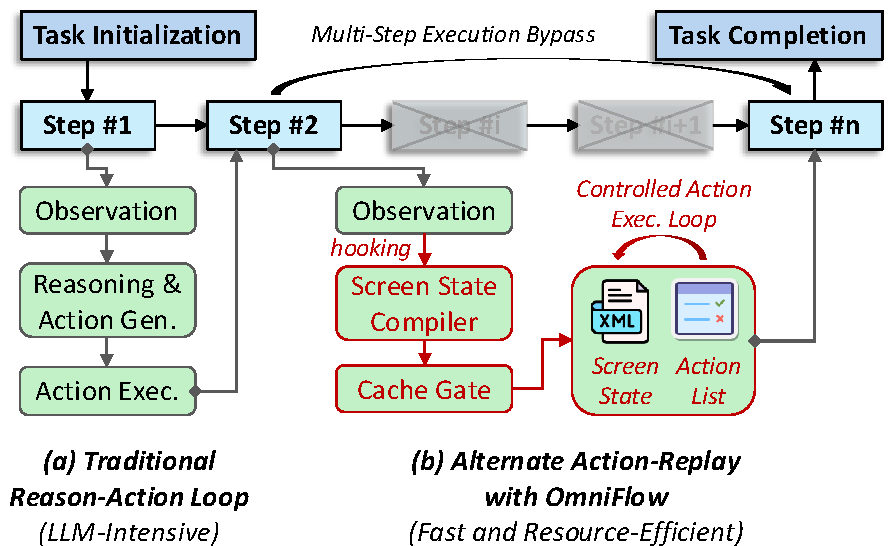
\includegraphics[width=0.45\textwidth]{figs/F14_comparison.pdf}
  \caption{Overview of \sysname workflow.
  The framework dynamically alternates between a traditional LLM-intensive reason-action loop (a) and a fast action-replay mechanism (b) to accelerate task execution.
  By hooking observations and querying the memory, the system recognizes familiar screen states and adaptively replays a cached list of atomic actions.}
  \label{fig:intro-comparison}
\end{figure}

\subsection{High Execution Costs of GUI Agents}
\label{sec:obs1}
\label{sec:obs2}

Mobile GUI agents typically operate in an observe--reason--act loop~\cite{rawles2025androidworld,wen2024autodroid,zhang2025appagent,wang2023enabling}.
As shown in Figure~\ref{fig:intro-comparison}, at each step, the agent perceives the current screen, invokes an LLM or VLM to determine the next GUI action, and executes the action in the environment.
Although this workflow enables flexible reasoning over open-ended tasks, it introduces substantial runtime overhead because model inference is repeatedly triggered during long interaction sequences.
The cost accumulates with each additional step, leading to increased latency and computation during task execution~\cite{dai2025advancing,zhang2025does,abhyankar2025osworld,zhong2026actionengine,zhang2025ufo2}.
Prior work reports that existing mobile agents often require more than 10 seconds per step, 1--2 minutes, and about \$1 monetary cost per task on average~\cite{dai2025advancing,christianos2025lightweight}.
More broadly, planning and reflection alone can account for 75\%--94\% of end-to-end latency in GUI agents~\cite{abhyankar2025osworld}.
These costs become more pronounced when the step-wise model inference runs directly on mobile devices with strict memory, power, and thermal constraints~\cite{dai2025advancing,christianos2025lightweight,zhang2024large}.

However, real-world mobile usage rarely consists of purely open-ended tasks.
In practice, users repeatedly perform similar routines, such as checking routine information, retrieving specific content, completing fixed navigation paths, and filling structured form-like workflows.
Prior studies characterize smartphone interaction as highly habitual, with repetitive checking behavior and app-launch patterns that are strongly shaped by recurring contexts such as time and location~\cite{oulasvirta2012habits,yan2012fast}.
Public mobile GUI datasets and benchmarks also reflect a similar pattern.
For example, the largest scale mobile GUI dataset to date, AITW, contains 715K episodes but only around 30K unique instructions~\cite{rawles2023android}.
We further quantify recurrence over the 30,378 subset-level unique-prompt entries reported across AITW's five subsets (Appendix~\ref{app:aitw-prompt-similarity}).  Parameter masking alone finds a template peer for 11,052 prompts (36.4\%).  Under a conservative criterion that accepts either a shared parameter template or semantic similarity of at least 0.98 while rejecting opposite intents, 22,834 prompts (75.2\%) have at least one similar counterpart; lowering the semantic threshold to 0.95 raises the estimate to 86.9\%.  These prompt-level rates estimate the workload available to a Function cache: they characterize candidate reuse demand, while executable Function reuse additionally requires compatible GUI state, action transfer, and terminal-effect verification.
Therefore, although per-step reasoning for open-ended tasks is crucial for high task completion rates, many realistic mobile-agent workloads are better viewed as repeated executions of recurring workflow patterns.

\zl{[This paragraph is the limitations of existing replay mechanisms; it also introduces massive new concepts such as coordinate replay and selector replay, which have not been introduced ahead.]}
This reuse problem is constrained by the observation interface itself.
Mobile GUI agents usually observe a screenshot, an Android accessibility tree, or both.
The accessibility tree reliably exposes element bounds and hierarchy when elements are observable, while semantic attributes such as \texttt{resource-id}, \texttt{text}, and \texttt{content-desc} only appear when developers provide them.
As a result, repeated execution cannot assume that every target has a stable selector: coordinate replay breaks under device-size and layout changes, and selector replay fails on missing annotations, custom-rendered widgets, WebViews, obfuscated resource identifiers, and unlabeled container controls.
The same instability limits graph-level reuse.
A conventional UI transition graph provides a useful state structure, but its nodes are often tied to raw XML or unstable attributes, and its edges record dispatched actions and state transitions rather than verified task effects.
\wzw{}{The missing object is a callable transition: a UTG edge can record that one action once moved an app from one observed state to another, but it does not by itself package runtime arguments, source-context transfer, or terminal/effect verification as an API-like operation.}
Such a graph is therefore difficult to reuse as a cross-device and cross-user execution cache under dynamic layouts and user-specific content.

\begin{table}[t]
  \centering
  \caption{Execution acceleration methods for mobile GUI agents.
  The columns capture whether a method (1) requires prior exploration on GUI states, (2) utilizes a cached memory without
  invoking LLM/VLM again, and (3) transfers its memory to dynamic and heterogeneous execution environments.}
  \label{tab:comparison}
  \resizebox{\columnwidth}{!}{
  \begin{tabular}{@{}lccc@{}}
  \toprule
  \textbf{Method}
    & \textbf{\begin{tabular}[c]{@{}c@{}}W/ App\\Exploration\end{tabular}}
    & \textbf{\begin{tabular}[c]{@{}c@{}}W/ Model\\Invocation\end{tabular}}
    & \textbf{\begin{tabular}[c]{@{}c@{}}Cross-Env\\Transferability\end{tabular}} \\
  \midrule
  RPA/script replay~\cite{li2017sugilite,gomez2013reran,maestro2026,openatx_uiautomator2_2026}
    & \cmark & \xmark & \xmark \\
  Memory-based~\cite{wen2024autodroid,zhang2025appagent,lee2024mobilegpt}
    & \cmark & \cmark & \xmark \\
  Program-guided~\cite{autodroid-v2,zhong2026actionengine,wang2026imperative,tian2025agentprog}
    & \cmark & \xmark & \xmark \\
  Per-step acceleration~\cite{dai2025advancing,lin2025showui,chen2025less,ouyang2026focusui}
    & \xmark & \cmark & \xmark \\ \hline
  \textbf{\sysname}
    & \textbf{\xmark} & \textbf{\xmark} & \textbf{\cmark} \\
  \bottomrule
  \end{tabular}
  }
\end{table}


\subsection{Reducing Runtime Costs}
\label{sec:bg-replay}
\label{sec:bg-programmatic}
\label{sec:bg-utg}

Prior studies on reducing the runtime costs of GUI agents primarily fall into several categories, which are summarized in Table~\ref{tab:comparison}.

\textbf{Robotic process automation (RPA)-based automation systems} treat mobile tasks as fixed workflows by recording and replaying user demonstrations~\cite{li2017sugilite,gomez2013reran,maestro2026,openatx_uiautomator2_2026}.
These systems construct replayable execution traces through human-driven app exploration before task execution.
However, the resulting memory is tightly bound to the recorded execution path, GUI layout, and entry state.
As a result, even minor changes in the live GUI state, such as screen modifications or layout updates, can cause the recorded execution to fail.

\textbf{Memory-based GUI agents} reduce runtime costs by reusing memory constructed from prior app exploration or first-time task execution.
For example, M3A~\cite{rawles2025androidworld} stores prior actions and their reasoning in prompts to guide later execution.
AutoDroid~\cite{wen2024autodroid} and AppAgent~\cite{zhang2025appagent} construct app-specific memory, such as UI transition graphs, through automated exploration and retrieve this memory during execution.
MobileGPT~\cite{lee2024mobilegpt} extends this idea with hierarchical app memory that stores reusable procedures and subtasks summarized from prior executions.
MobiMem~\cite{liu2025beyond} reduces repeated GUI-agent reasoning by reusing prior executions through experience memory, which abstracts task traces into reusable templates, and action memory, which caches low-level action sequences for direct replay.
\textbf{Program-guided agents}~\cite{autodroid-v2,zhong2026actionengine,wang2026imperative,tian2025agentprog} further reduce runtime costs by translating task knowledge or prior demonstrations into executable scripts.
These scripts allow repeated GUI operations to be completed through deterministic program execution with fewer model invocations.
Together, memory-based and program-guided agents replace parts of VLM-based step-wise action generation with previously validated memory or executable operations.
However, these methods still rely on memory constructed from prior app exploration, user interaction, or first-time execution, which can introduce privacy concerns and limit transfer across users, devices, app versions, and unseen environments.

% Related memory mechanisms have also been explored in AppAgentX, which identifies repetitive action sequences from execution history and compiles them into higher-level shortcuts~\cite{jiang2025appagentx}.
% \zl{AxNav~\cite{taeb2023axnav}, UINav~\cite{li2023uinav}, AutoTask~\cite{pan2023autotask}}

% Third, \textbf{program-guided agents} generate executable scripts or programs
% from collected app documentation, state-machine memory, or declarative
% interfaces~\cite{autodroid-v2,zhong2026actionengine,wang2026imperative,tian2025agentprog}.
% These systems improve long-horizon control, but they still rely on substantial
% app knowledge and online adaptation when the live state diverges from the
% stored program.

Another line of studies, \textbf{per-step inference acceleration methods}, retain the traditional observe--reason--act loop while reducing the cost of each individual decision.
V-Droid~\cite{dai2025advancing} replaces auto-regressive action generation with verifier-based ranking over a discretized action space, which substantially reduces latency.
ShowUI~\cite{lin2025showui} accelerates VLM inference through UI-guided visual token selection.
Other studies accelerate execution by pruning redundant visual or historical context before model inference, such as masking-based GUI element pruning, history compression~\cite{chen2025less}, and position-preserving UI token selection~\cite{ouyang2026focusui}.

To summarize, existing approaches still face several limitations.
RPA-based systems and script replay provide executable workflows, but they are fragile when the live GUI state diverges from the recorded execution.
Memory-based and program-guided agents reduce repeated reasoning, but they often rely on substantial app exploration and provide limited support for workflow-level adaptation.
Per-step inference acceleration methods reduce the cost of each individual decision, but they still require repeated VLM-based step-wise action generation in long interaction loops.
These limitations motivate us to build \sysname for generalizable memory reuse across dynamic app environments.

\subsection{Goals and Challenges}
\label{sec:obs3}
\label{sec:obs-need}

Mobile apps dynamically change across users, devices, and sessions and often lack stable APIs for GUI agents to invoke. While traces usually expose a fixed-action subspace:
within a ReAct loop, recurring tasks often contain high-frequency repeated
Functions, such as opening a search page, entering a query, filling a form, or
confirming a save.  We call such reusable units \texttt{Functions}.  This
observation suggests storing them as persistent Functions that can be updated over
time, so the agent can skip reasoning and execute directly when the same
situation recurs.

Our goal is to design a memory system for mobile GUI agents that can reuse past executions in dynamic app environments while allowing flexible switching between memory-guided execution and VLM-based step-wise action generation.
This requires memory to support both workflow-level adaptation, where the execution path may change, and state-level adaptation, where a memorized GUI state may appear differently from the live GUI state.


\textbf{Adaptive Reuse Workflow.}
The first challenge is representing past executions at a granularity suitable for flexible reuse.
Existing memory systems for GUI agents often store a complete long-horizon trajectory or split it into fixed subtasks, then guide the agent to follow the recorded execution path.
This design is fragile in real mobile apps, where workflows frequently change due to expired login sessions, pop-ups, loading delays, or permission dialogs.
A coarse-grained memory may fail even when most parts of the historical execution remain reusable.
This calls for a finer-grained memory representation that can reuse matched Functions while allowing the agent to fall back to VLM-based step-wise action generation when the live workflow diverges.

\textbf{Adaptive Action Grounding.}
The second challenge is applying a memorized operation to a live GUI state safely.
Even when the live GUI state corresponds to a memorized GUI state, the target GUI component may shift due to screen size, font scale, list ordering, or dynamic content.
This requires the system to be able to utilize historical context to achieve localization enhancement.

\begin{table}[t]
  \centering
  \caption{Execution costs of different on-device inference backends.We use Qwen-vl-0.8B-W4A16 on OnePlus 12.}
  \label{tab:ondevice-cost}
  \resizebox{\columnwidth}{!}{%
  \begin{tabular}{llllr}
    \toprule
    Location & Backend & Input & Tokens & Time \\
    \midrule
    On-device & Llama.cpp & screenshot & $\sim$2,500 & 60\,s+ \\
    On-device & MNN-LMM  & screenshot & $\sim$2,500 & 10\,s+ \\
    Cloud     & Qwen-API  & screenshot & $\sim$3,200 & 3\,s  \\
    \bottomrule
  \end{tabular}}
\end{table}
